
\chapter{ Movimento de um corpo em queda vertical: determinação da aceleração da queda } \\

\vspace{-0.7cm}

\section{Introdução}
Neste experimento determinaremos a aceleração de um corpo em queda vertical e vamos 
comparar o resultado obtido com o valor de referência da aceleração da gravidade ($g$)
para a cidade de Rio de Janeiro. 
\par
Vamos analisar o movimento de queda vertical de um corpo cuja forma e tamanho apresente uma força de resistência do ar desprezível (por exemplo uma bolinha de gude)\footnote{Lembre que a queda vertical de um corpo quando a única força atuante sobre ele é a força da gravidade chama-se queda livre.}. Que tipo de movimento 
apresentaria o corpo se a força de resistência do ar fosse desprezível?\footnote{Lembre que o movimento da partícula é determinado através da Segunda Lei de Newton.}
\par 
Pense sobre o planejamento desse experimento. A aceleração do corpo pode ser obtida diretamente? Quais grandezas devem ser medidas para que seja possível obtê-la? Quais instrumentos são mais adequados para que esses dados possam ser coletados?
\par 
O experimento será discutido e guiado pelo roteiro abaixo. Siga o roteiro e as orientações do professor 
nos encontros remotos e vá fazendo suas anotações no caderno de laboratório. 

% ----------------------------------------------------------------------------
\section{Procedimento Experimental}
% ----------------------------------------------------------------------------

\begin{minipage}[c]{11.5cm}

\hskip 0.5cm
O arranjo experimental experimental está mostrado na Figura~\ref{fig:experimento}. Escolha uma bola de gude ou qualquer corpo arredondado de dimensões da ordem de grandeza da bolinha mostrada na Figura~\ref{fig:experimento}. Você deverá filmar a queda da bolinha com um celular, desde uma altura de, mais o menos, um metro. Para isso peça ajuda a uma pessoa que vai segurar a bolinha enquanto você filma.  Cole na parede uma régua de papel como está indicado na Figura \footnote{A régua não precisa ter a extensão de toda a trajetória a ser filmada. É somente uma referencia de escala.}. Para a filmagem posicione o celular num apoio com a tela do celular paralela à parede onde está colada a régua de papel. O celular deverá estar posicionado mais o menos no meio da trajetória da bolinha a uma distância da parede suficiente para poder filmar toda a queda de mais ou menos um metro. Não use ``slow-motion'' (câmera lenta),  filme com a velocidade normal do seu celular. A imensa maioria dos celulares filma a uma taxa de 30 frames/seg \footnote{A palavra em inglês ``frame'' significa quadro.}. Verifique no seu celular se essa é a taxa usada.
\par
\hskip 0.5cm
Para analisar o filme da queda será usado o aplicativo Tracker para uso num computador 
que poderá ser baixado gratuitamente no endereço eletrônico: \break  {\color{blue} https://physlets.org/tracker/} \footnote {O aplicativo é disponibilizado para os sistemas operacionais Windows, Linux e Mac OSX.}. Alternativamente o filme poderá ser analisado com o aplicativo VidAnalysis disponível gratuitamente para celulares com sistema operacional Android no link  {\color{blue} https://play.google.com/store/apps/details?id=com.vidanalysis.free}. 
Os tutoriais de uso destes aplicativos estão disponíveis na forma de vídeos no site da disciplina dentro do site do Instituto de Física da UFRJ. No final do roteiro, encontram-se o Apêndice \ref{ApendiceB} um tutorial básico do aplicativo Tracker, e um tutorial básico do aplicativo VidAnalysis no Apêndice \ref{ApendiceC}.  
\end{minipage}
\hskip 0.2cm
\begin{minipage}[c]{7cm}
\hskip 1cm
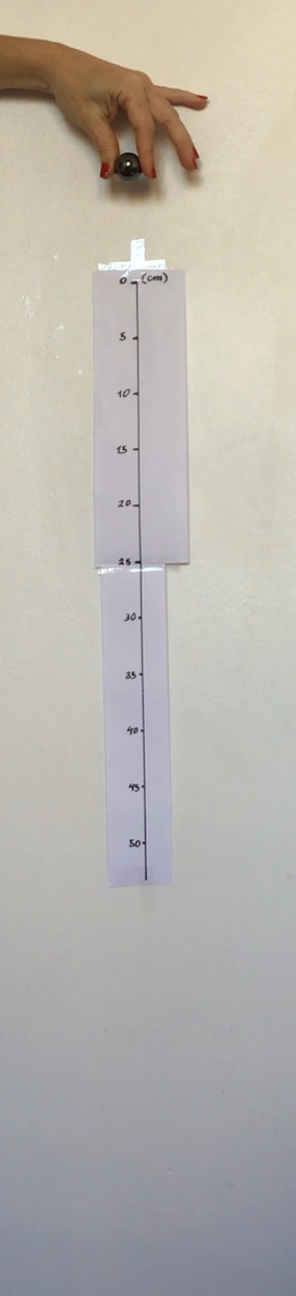
\includegraphics[width=4.5cm]{Figuras_exp3/fig1.pdf}
\caption{figure}{\label{fig:experimento} Dispositivo experimental. Não esqueça de colar na parede uma régua de papel, como a indicada na Figura, para ser usada como referência na análise de dados.}
%\label{fig1}
\end{minipage}
\clearpage
% ----------------------------------------------------------------------------
\section{Análise de dados}
% ----------------------------------------------------------------------------
\indent 


Usando o aplicativo Tracker ou alternativamente o aplicativo  VidAnalysis, monte a Tabela \ref{tabela1}.
\begin{table}[h!]
\centering
\begin{tabular}{c|c|c|c|c}
t (s) & $y$ (cm) & $\delta y$ (cm)& $v_y$ (cm/s)& $\delta v_y$ (cm/s)\\
\hline 
&&&& 
\end{tabular}
\caption{Tabela de dados da experiência.}
\label{tabela1}
\end{table}
\par
\begin{minipage}[c]{11.5cm}
\hskip 0.5cm
As colunas do tempo $t$ e da posição $y$ são preenchidas usando os aplicativos Tracker 
ou  VidAnalysis. As coordenadas $y$ correspondem às posições, por exemplo, do centro da bolinha ao longo da trajetória de queda, após ter escolhido o sistema de referência. Note que ao longo da trajetória a imagem da bolinha pode ficar um pouco embaçada como na Figura~\ref{fig:reguacomxis}. 
Nesse caso, foi marcado com um "x"  em azul 
o centro da bolinha enquanto que a barra vermelha é uma escolha razoável da região de incerteza
da posição do centro da bolinha.  
\par
\hskip 0.5cm
Para preencher a coluna da velocidade $v_y$ leia o Apêndice \ref{ApendiceD} (no final do roteiro).
Como são calculadas as incertezas $\delta v_y$?
\par 
%\hskip 0.5cm
\begin{itemize}
\item Em papel milimetrado desenhe o gráfico $v_y$ vs. $t$ a partir dos dados da tabela indicando 
a incerteza nos valores das velocidades. Qual é a forma esperada para este gráfico?
\item Use as colunas $t$, $v_y$ e $\delta v_y$ para  calcular através do Método dos Mínimos Quadrados (Seção I.5  de Conceitos básicos da Apostila) qual é a melhor reta que aproxima os dados experimentais do gráfico $v_y$ vs. $t$. 
\end{itemize}
\end{minipage}
\hskip 0.2cm
\begin{minipage}[c]{6cm}
%%%%%%%%%%%%%%%%%%%%%%%%%%%%%%%%
%\begin{figure}[h!]
%\centering
\hskip 1cm
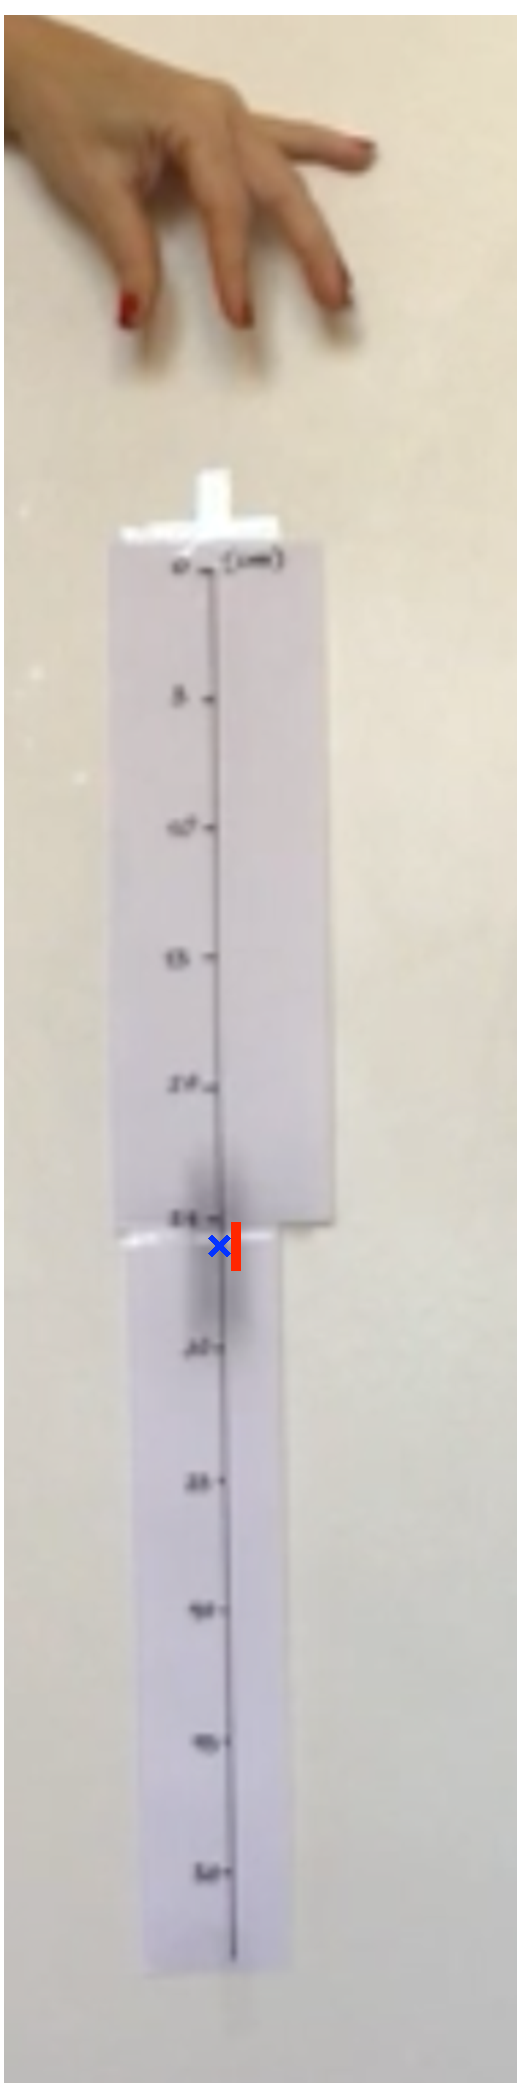
\includegraphics[width=3.8cm]{Figuras_exp3/fig2roteiro.pdf}
\captionof{figure}{\label{fig:reguacomxis} Imagem da bolinha em plena queda. Note-se que a imagem, devido à alta velocidade, fica um pouco embaçada.}
\label{fig2roteiro}
%\end{figure}
%%%%%%%%%%%%%%%%%%%%%%%%%%%%%%%%
\end{minipage}
\begin{itemize}
\item Com os parâmetros da reta obtida no item anterior,  desenhe-a  na mesma folha de papel milimetrado 
onde fez o gráfico $v_y$ vs. $t$. Se você não conseguir um aplicativo que implemente o ajuste linear pelo método dos mínimos quadrados desenhe a melhor reta que aproxima os dados experimentais 
pelo método visual (ver o Apêndice \ref{ApendiceG}) e obtenha os parâmetros que definem a reta 
(inclinação $a$ e coeficiente linear $b$) escolhendo dois pontos na reta e substituindo na equação da reta $y=a\;t+b$.
\end{itemize}
  
\clearpage

% ----------------------------------------------------------------------------
\section{Discussão dos resultados}
% ----------------------------------------------------------------------------

\begin{enumerate}
\item A partir dos parâmetros do ajuste linear aos dados experimentais $v_y$ vs. $t$, 
como se obtêm o valor da aceleração de queda da bolinha?
\item 
Compare o valor da aceleração de queda da bolinha com o valor da aceleração da gravidade 
para a cidade do Rio de Janeiro que é $g=(978,7\pm 0.1)$ cm/$s^2$). 
Qual valor é mais preciso? Você utilizaria este método para determinar o valor da gravidade? Justifique.
\end{enumerate}
\par 
No relatório você deverá entregar um arquivo pdf que
contenha o objetivo do experimento, a Tabela \ref{tabela1} e o gráfico em papel milimetrado dos dados experimentais de $v_y$ vs. $t$ assim como o ajuste linear. Também deverá entregar nesse arquivo pdf  a discussão dos ítens 1 e 2 acima. 

\section{Opcional: Estudo da conservação da energia}
\indent

Também poderá entregar no arquivo pdf do relatório as seguintes tarefas opcionais:

\begin{enumerate}
\item Utilizando os dados registrados para a posição $y$ como função do tempo $t$, determine a altura $h$ da bolinha para cada instante de tempo, a partir do ponto mais baixo na Tabela~\ref{tabela1}.
\item Determine a energia cinética ($K$), energia potencial ($U$) e a energia mecânica ($E$) para cada intervalo de tempo. Para facilitar a organização das informações, construa uma tabela.
\item Faça um gráfico que contenha a energia cinética, potencial e mecânica em função do tempo.
\item Discuta a partir do gráfico obtido, se há ou não conservação da energia mecânica. Justificar.
\item No caso da energia não se conservar, determine o ganho ou perda percentual.
\end{enumerate}
\underline{\bf Observações:}
\\
\begin{itemize}
\item Para os cálculos de energia considere a aceleração da gravidade no Rio de Janeiro, 
sendo $g=(978,7\pm 0,1)$ cm/$s^2$).
\item Não esqueça de colocar todos os cálculos de propagação de incerteza num Apêndice.
\end{itemize}

\clearpage

\appendix
 %-----------------------------------------------------------------------------------------------------------------
\section{Apêndice A: Movimento Retilíneo Uniformemente Variado (MRUV)}
\label{ApendiceA}
 %-----------------------------------------------------------------------------------------------------------------
\indent

Se a força resultante sobre uma partícula de massa $m$ for, $\vec{F}$, a  segunda lei de Newton diz que:
\begin{equation}
\label{eqA1}
\vec{F}=m\vec{a},
\end{equation}
com $\vec{a}$ sendo o vetor aceleração da partícula. No caso de $\vec{F}$ ser uma força constante,
{\it viz.} não depende nem do tempo, nem da posição da partícula e nem da velocidade da mesma, da Eq.(\ref{eqA1}) vemos que 
a aceleração $\vec{a}$ é constante. Assim, a Eq.(\ref{eqA1}) pode ser facilmente integrada para obtermos:
\begin{equation}
\label{eqA2}
\int_{t_0}^{t}\vec{F}dt=m\int_{t_0}^{t} \vec{a}dt\Longrightarrow \vec{F}(t-t_0)=m(\vec{v}-\vec{v}_0)
\Longrightarrow \vec{v}=\vec{v}_0+\frac{\vec{F}}{m} (t-t_0),
\end{equation}
com $\vec{v}:=\vec{v}(t)$ e $\vec{v}_0:=\vec{v}(t_0)$.
Integrando temporalmente mais uma vez ambos os membros da Eq.(\ref{eqA2}) obtemos:
\begin{equation}
\vec{r}=\vec{r}_0+\vec{v}_0(t-t_0)+\frac{1}{2}\frac{\vec{F}}{m}(t-t_0)^2,
\end{equation}
com $\vec{r}:=\vec{r}(t)$ sendo a posição da partícula como função do tempo e 
$\vec{r}_0:=\vec{r}(t_0)$ a sua posição inicial.
\par
Vamos supor agora que a força resultante 
$\vec{F}$ é paralela à velocidade inicial $\vec{v}_0$. Como a soma vetorial de vetores paralelos 
continua sendo um vetor na mesma direção que os vetores somados, de acordo com a Eq.(\ref{eqA2}), a velocidade $\vec{v}(t)$ é paralela a $\vec{v}_0$ para todo tempo. Portanto trata-se 
de um movimento retilíneo. Como também a aceleração é constante o movimento se denomina 
Movimento Retilíneo Uniformemente Variado (MRUV). Sem perda de generalidade podemos 
chamar de eixo ``$y$'' o eixo coordenado na direção de movimento,  e as equações de movimento,  Eqs.(\ref{eqA1}) e (\ref{eqA2}), nessa direção são:
\bea
y&=&y_0+v_{y0}(t-t_0) +\frac{1}{2} \frac{F}{m}(t_0)^2,\\
v_y&=&v_{y0}+\frac{F}{m}(t-t_0),
\eea 
com $y:=y(t)$ e $v_y:=v_y(t)$ e as condições iniciais, $y_0:=y(t_0)$ e $v_{y0}:=v_y(t_0)$.


